\chapter{计算CTL下的遗忘:基于归结的方法}\label{chapter04}
{\em 
已有结果显示,任意的$\CTL$公式可以转换为$\CTLsnf$子句的集合。归结是一种以子句为计算对象的判断可满足性的方法,本章提出一种基于归结的计算遗忘的方法。
其主要思想是:首先将给定的$\CTL$公式转换为$\CTLsnf$子句的集合(这一部分在第\ref{chapter02}章已经给出了详细的介绍),其次在相应的原子命题集合$V$上使用归结规则得到归结结果,最后“消除”之前引入的索引和$\start$,最终得到遗忘的结果。其主要流程图如图\ref{Fig:chapter05:v1uv2}所示。
正如本章所要说明的那样,$\CTL$不具有均匀插值这一属性,基于归结的方法在有的情况下是不能计算出遗忘结果的。然而,在有些$\CTL$子类下,本章提出的方法能够计算出其遗忘结果。}
\begin{figure*}[!htb]
	\centering
	% Requires \usepackage{graphicx}
	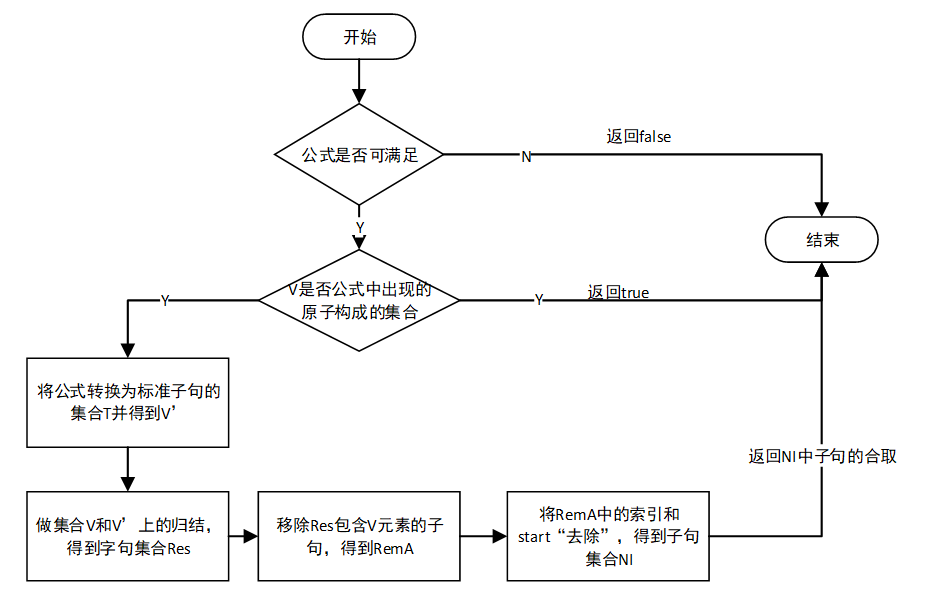
\includegraphics[width=15cm]{chapter04/frame.png}\\
	\caption{基于归结的遗忘的主要流程图}
	\label{Fig:chapter05:v1uv2}
\end{figure*}

\section{引言}
虽然在第\ref{chapter02}章详细介绍了命题逻辑和模态逻辑S5下基于归结的计算遗忘的方法,但值得注意的是$\CTL$公式没有像这两种逻辑一样有标准的自身语言子句形式,而$\CTL$的子句是有索引的。这就注定了$\CTL$下基于归结的遗忘与上述两者的不同,而且也应该要复杂一些(虽有不同,但也可以借鉴)。
本章展示如何使用第\ref{chapter02:CTLres}节中表\ref{tab:res}中的归结规则来计算$\CTL$下的遗忘。

%在本章给定如下约定的记号。令$V\subseteq \Ha$是要遗忘的原子命题的集合,$I\subseteq \Ind$是索引的集合,$V'$表示计算过程所引入的原子命题的集合且满足$V'\cap V=\emptyset$。
%此外,$\varphi$是$\CTL$公式,且$T_{\varphi}$是在$\varphi$上使用表\ref{tab:trans}中的转换规则得到的$\CTLsnf$子句的集合。
%显然可以知道,$V'=\Var(T_{\varphi})-\Var(\varphi)$。
%在不另加说明的情况下$\Hm$表示五元组$(S,R,L,[\_],s_0)$。
%此时,本章所设计的算法的伪代码如算法\ref{alg:compute:forgetting:by:Resolution}所示。



%算法\ref{alg:compute:forgetting:by:Resolution}对于输入$\varphi$和$V$,输出结果记为$ERes(\varphi, V)$。
为了计算从$\CTL$公式$\varphi$中遗忘掉集合$V$中的原子命题,
%为了实现这一目标,
需要解决如下两个主要问题:
\begin{itemize}
	\item[(1)] 如何表示$\CTL$公式和带索引的$\CTL$公式之间的关系?如在第\ref{chapter02}章中所展示的那样,将一个$\CTL$公式转换为$\CTLsnf$子句的集合会引入新的原子命题和索引。虽然已有的研究说明了$\CTL$公式可以转换为带索引的公式的集合并保证其可满足性,然而并没有表明这两种形式的公式之间的模型具有怎样的联系。
	本章从互模拟等价的角度探讨$\CTL$公式和归结等过程得到的(带索引)公式之间的联系,为计算遗忘提供理论基础。
	%本章给出一种扩展的互模拟定义,以描述两种公式的模型之间的关系。
	\item[(2)] 如何“移除”无关的原子命题(包括需要遗忘的原子命题和转换过程中引入的新的原子命题),以及如何“消除”索引?为此,本章给出“移除”原子命题的一般操作,并提出一种一般化的Ackermann引理。为了“消除”索引,探索几个逻辑等价关系,详见第\ref{cha4:sec:resf}节。
	%对应算法\ref{alg:compute:forgetting:by:Resolution}中的$\emph{Removing\_index}(\emph{RemA})$过程。
\end{itemize}

本章其余部分组织如下:首先,第\ref{cha4:sec:resf}节给出归结过程的详细介绍。其次,第\label{cha4:sec:reIndex}节介绍如何将第\ref{cha4:sec:resf}节得到的结果转换成$\CTL$公式,具体分为两部分:移除索引和移除新引入的原子命题。第\ref{cha4:sec:alg}节给出计算遗忘的算法,并分析算法的时间和空间复杂性。最后总结本章的主要工作。



%\section{二元互模拟}
%\label{chapter4:sub:biVB}
%对于给定的初始$\Ind$-结构,这里定义一种$\tuple{V, I}$-互模拟关系。为了与一元的(只考虑原子命题的集合)$V$-互模拟对应,称$\tuple{V, I}$-互模拟为二元互模拟。其在$V$-互模拟的基础上又考虑了索引的集合在结构间关系。
%\begin{definition}[二元互模拟] \label{def:VInd:bisimulation}
%	令$V\subseteq \Ha$、$I\subseteq \Ind$分别是原子命题和索引的集合,${\cal K}_i=(\Hm_i,s^i)$是初始$\Ind$-结构,其中$\Hm_i=(S_i, R_i, L_i, [\_],s_0^i)$ $(i=1,2)$。称${\cal K}_1$和${\cal K}_2$是 $\tuple{V, I}$-互模拟的(记为${\cal K}_1 \lrto_{\tuple{V, I}} {\cal K}_2$),当且仅当${\cal K}_1 \lrto_V {\cal K}_2$且$\forall j\in (\Ind - I)$有:
%	\begin{itemize}
%		\item 对任意的$(s,s_1) \in [j]_1$,存在$(s',s_1')\in [j]_2$使得$s\lrto_V s'$且$s_1 \lrto_V s_1'$;
%		\item 对任意的$(s',s_1') \in [j]_2$,存在$(s,s_1)\in [j]_1$使得$s\lrto_V s'$且$s_1 \lrto_V s_1'$。
%	\end{itemize}
%	
%\end{definition}
%
%由定义\ref{def:VInd:bisimulation}可知,当探讨的公式为$\CTL$公式时,因为不用考虑索引,$\lrto_{\tuple{V, I}}$“降维”为$\lrto_V$。
%与$\lrto_V$类似,$\lrto_{\tuple{V, I}}$在本文中至关重要的两个性质如下。
%\begin{proposition}\label{pro:VI:div}
%	令$V_1,V_2\subseteq \Ha$为原子命题的集合,$I_1, I_2 \subseteq \Ind$为索引的集合,${\cal K}_i = (\Hm_i, s_0^i)$ $(i=1,2,3)$为初始$\Ind$-结构。若${\cal K}_1 \lrto_{\tuple{V_1,I_1}} {\cal K}_2$、${\cal K}_2 \lrto_{\tuple{V_2,I_2}} {\cal K}_3$,则:
%	\begin{itemize}
%		\item[(i)] ${\cal K}_1 \lrto_{\tuple{V_1\cup V_2,I_1\cup I_2}} {\cal K}_3$;
%		\item[(ii)] 如果$V_1 \subseteq V_2$且$I_1 \subseteq I_2$,则${\cal K}_1 \lrto_{\tuple{V_2,I_2}} {\cal K}_2$。
%	\end{itemize}
%\end{proposition}
%\begin{proof}
%	(i) 由定义\ref{def:VInd:bisimulation}可知${\cal K}_1 \lrto_{V_1} {\cal K}_2$、${\cal K}_2 \lrto_{V_2} {\cal K}_3$,因此由命题\ref{pro:div}可知${\cal K}_1 \lrto_{V_1\cup V_2} {\cal K}_3$。
%	
%	${\cal K}_1 \lrto_{\tuple{V_1,I_1}} {\cal K}_2$\\
%	$\Rto$ $\forall j\in (\Ind-(I_1\cup I_2))$有:$\forall(s,s_1) \in [j]_1$,$\exists (s', s_1')\in [j]_2$使得$s\lrto_{V_1} s'$,$s_1\lrto_{V_1} s_1'$\\
%	$\Rto$ 又因为${\cal K}_2 \lrto_{\tuple{V_2,I_2}} {\cal K}_3$,所以$\exists (s'', s_1'')\in [j]_3$使得$s'\lrto_{V_2} s''$,$s_1'\lrto_{V_2} s_1''$  \hfill \\
%	$\Rto$ $s \lrto_{V_1\cup V_2} s''$且$s_1 \lrto_{V_1\cup V_2} s_1''$
%	
%	同理可证,$\forall (s'',s_1'')\in [j]_3$,$\exists (s,s_1)\in [j]_1$使得$s \lrto_{V_1\cup V_2} s''$且$s_1 \lrto_{V_1\cup V_2} s_1''$。
%	因此,由定义\ref{def:VInd:bisimulation}可知${\cal K}_1 \lrto_{\tuple{V_1\cup V_2,I_1\cup I_2}} {\cal K}_3$。
%	
%	(ii)可以由命题\ref{pro:div}中的(ii)可得。
%\end{proof}
%
%对于给定的$\Ind$-Kripke结构$\Hm=(S,R,L,[\_],s_0)$和$\Hm'=(S',R',L',[\_],s_0')$,$\Hm$和$\Hm'$之间的二元互模拟关系$\lrto_{\tuple{V,I}}$给描述公式间在二元组$\tuple{V,I}$上的等价关系提供了前提条件。这同时也为解决本章引言部分提出的问题$(1)$奠定了基础。
%
%\begin{definition}
%	给定两个公式(或公式的集合)$T_1$和$T_2$,$I\subseteq \Ind$是索引的集合,$V''\subseteq \Ha$是原子命题的集合。如果下面条件被满足,则称$T_1$和$T_2$在二元组$\tuple{V,I}$上逻辑等价(记为$T_1\equiv_{\tuple{V,I}} T_2$):
%	\begin{itemize}
%		\item $\forall (\Hm,s_0)\in \Mod(T_1)$,$\exists (\Hm',s_0')\in \Mod(T_2)$使得$(\Hm,s_0) \lrto_{\tuple{V, I}} (\Hm',s_0')$,且
%		\item $\forall (\Hm',s_0')\in \Mod(T_2)$,$\exists (\Hm,s_0)\in \Mod(T_1)$使得$(\Hm,s_0) \lrto_{\tuple{V, I}} (\Hm',s_0')$。
%	\end{itemize}
%	
%\end{definition}



\section{$\CTL$归结$\Unfolding$}
\label{cha4:sec:resf}
这部分给出如何使用归结规则(表\ref{tab:res})来计算$\CTL$中的遗忘。
这个过程的主要思想是将转换过程中获得的$\CTLsnf$子句在表\ref{tab:res}中归结规则上做穷尽的归结,即直到不产生新的归结结果。值得注意的是该归结过程涉及的归结原子命题是需要遗忘的和转换过程中引入的新的原子命题,这是与判定可满足性下做所有原子命题的归结的不同。

令$T$为$\CTLsnf$子句的集合,$p$为原子命题。$T$在$p$上的\emph{展开}(记为$\Unfolding(T,p)$)是集合$T$和如下集合的并集:
\[\{\alpha\mid \mbox{$\alpha$ 是 $T$ 中的公式关于文字 $l\in\{p,\neg p\}$ 的归结结果}\}.  \]
对于原子命题的集合$V$,定义$\Unfolding(T,\emptyset)=T$且$\Unfolding(T,\{p\}\cup V)=\Unfolding(\Unfolding(T,p), V)$。
直观地说,$T$在$p$上的展开是对$p$做穷尽的归结,也就是直到对$p$使用规则{\bf SRES1-8}不再产生新的$\CTLsnf$子句为止(即使使用了重写规则和可能规则之后也不会产生新的子句)。


下面的命题展示了对任意的$\CTL$公式$\varphi$,从 $\Unfolding(T_\varphi,V)$ 中移除掉含有$V$中元素的子句得到的结果在不考虑$V$中元素和新引入的元素的情况下是互模拟等价的。
下文中记$\emph{ERes}(\varphi,V) = \{\alpha\in \Unfolding(T_\varphi,V)\mid \Var(\alpha)\cap V=\emptyset\}$。
\begin{proposition}\label{pro:resEQ}
	令 $\varphi$ 为一个 $\CTL$公式,$V\subseteq\cal A$为原子命题的集合。则
	$T_\varphi \equiv_U\emph{ERes}(\varphi,V)$,其中  $U=\Var(\Unfolding(T_\varphi,V))-(\Var(\varphi)-  V)$。
\end{proposition}
	\begin{proof}
	从两个方面来证明这一结论:\textbf{(F1)} $T_\varphi \equiv_U \Unfolding(T_\varphi,V)$, \textbf{(F2)} $\Unfolding(T_\varphi,V) \equiv_{U} \emph{ERes}(\varphi,V)$。
	为了方便,定义如下 由$\CTLsnf$ 子句集合构成的序列: $T_0=T_{\varphi}, T_1, T_2, \dots, T_n = \Unfolding(T_\varphi,V)$,其中
	$T_{i+1} = T_i \cup R_i$ ($0\leq i < n$)、 $R_i$ 是对$\Pi \subseteq T_i$使用一条匹配的规则$r$且该规则归结的原子命题为$p\in V$,这一过程记为 $\Pi \rto_r R_i$。
	\\
	
	\textbf{(F1)} 为了证明$T_\varphi \equiv_U \Unfolding(T_\varphi,V)$,这里证明 对任意的 $0\leq i < n$ 有$T_i \equiv_{U} T_{i+1}$。
	
	
	
	(1) 若 $r\in \{\textbf{(SRES1)},$ $\dots,$ $\textbf{(SRES8)},$ $(\textbf{RW1}),$ $(\textbf{RW2})\}$,则$T_i \equiv_{\{p\}} T_{i+1}$,其中。
	
	
	一方面,显然 $\Pi \models R_i$,所以 $T_i \models T_{i+1}$。另一方面 $T_i\subseteq T_{i+1}$,所以 $T_{i+1} \models T_i$。
	
	(2) 这里证明若$\Pi \rto_r R_i$且 $r=$\textbf{(ERES1)},
	则 $T_i \equiv_{\{l, w_{\neg l}^{\ALL}\}} T_{i+1}$,其中 $l = p$或 $l = \neg p$,$w_{\neg l}^{\ALL}$是与子句$Q \rto \ALL \FUTURE \neg l$相关的新的原子命题,$l$是文字(即:$p$或者$\neg p$)。
	
	在文章~\cite{bolotov2000clausal}中已经证明$\Pi \models R_i$,因此有$T_{i+1}=T_i \cup \Lambda_{\neg l}^{\ALL}$,其中$\Lambda_{\neg l}^{\ALL}$是通过使用表\ref{tab:trans}中的转换规则作用到$R_i$上得到的$\CTLsnf$子句的集合(请查看文章~\cite{zhang2009refined}获取更加详细的描述)。显然,对所有的$(\Hm_1,s_1) \in \Mod(T_i= X \cup \Pi)$都存在一个$(\Hm_2, s_2)\in \Mod(T_{i+1}=T_i \cup \Lambda_{\neg l}^{\ALL})$使得$(\Hm_1, s_1) \lrto_{\tuple{\{p, w_{\neg l}^{\ALL}\}, {\O}}} (\Hm_2, s_2)$,且对任意的$(\Hm_2, s_2)\in \Mod(T_{i+1}=T_i \cup \Lambda_{\neg l}^{\ALL})$也存在一个$(\Hm_1,s_1) \in \Mod(T_i= X \cup \Pi)$使得$(\Hm_1, s_1) \lrto_{\{p, w_{\neg l}^{\ALL}\}} (\Hm_2, s_2)$。
	又$\{p, w_{\neg l}^{\ALL}\} \subseteq U$,由命题\ref{prop:transform:V:EQ}可知$T_i \equiv_{U} T_{i+1}$。
	
	当规则为$\textbf{(ERES2)}$时可以类似地证明。
	
	总之,$V\subseteq U$,因此由推论\ref{cor:eqbi}(iii)可知对任意的 $0 \leq i < n$ 有$T_i \equiv_U T_{i+1}$。
	又因为$\equiv_U$为一个等价关系,所以$T_{\varphi} \equiv_U \Unfolding(T_\varphi,V)$。
	
	
	
	\textbf{(F2)} 不失一般性地,假设 $V=\{p\}$, $C_i$ ($i=1,2$)为经典子句,  $l = p$ 或 $l = \neg p$。
	显然 $\Unfolding(T_\varphi,V) \models \emph{ERes}(\varphi,V)$,这里证明对任意的 ${\cal K}=(\Hm, s)\in \Mod(\emph{ERes}(\varphi,V))$ (其中$\Hm=(S, R, L, [\_], s)$),存在一个初始$\Ind$-结构 ${\cal K}'=(\Hm', s')$ 使得 ${\cal K} \lrto_{U} {\cal K}'$ 且 ${\cal K}' \models \Unfolding(T_\varphi,V)$。
	
	
	因为$p$ 只出现在 $\CTLsnf$子句的右手边,这里从下面几点证明上述结论成立。
	
	(1) 假定 $\Unfolding(T_\varphi,V)$有全局子句,则对于任意的 $C=\top\rto C_1 \vee l \in \Unfolding(T_\varphi,V)$:
	
	(a) 如果不存在 $C'\in \Unfolding(T_\varphi,V)$ 使得 $C$ 和 $C'$ 在 $p$上是可归结的,则 $\Unfolding(T_\varphi,V)$中不存在除了 $Pt$-某时 子句之外的子句 $C'$ 包含文字 $\neg l$,其中 $Pt\in \{\ALL, \EXIST\}$。
	
	若对任意其他的子句$C'$, $p\not \in \Var(C')$,则对任意的 ${\cal K}=(\Hm, s)\in \Mod(\emph{ERes}(\varphi,V))$可如下构造 $(\Hm',s')$:令 $\Hm'= (S, R, L',[\_], s)$ (即 $s'=s$),其中$L'$ 与 $L$ 一样,除了对任意的 $s_1\in S$,若 $(\Hm, s_1) \not \models C_1 \vee l$则“若 $l=p$令 $L'(s_1) = L(s_1) \cup \{p\}$,否则令 $L'(s_1) = L(s_1) - \{p\}$”。
	显然 $(\Hm, s) \lrto_{\{p\}} (\Hm', s')$ 和 $(\Hm', s') \models C' \wedge C$。
	
	若 $C'= Q\rto Pt \FUTURE \neg l$,不失一般性地,令 $l=p$。对任意的 ${\cal K}=(\Hm, s)\in \Mod(\emph{ERes}(\varphi,$ $V))$,如下构造 $(\Hm',s')$:令$\Hm'=(S, R, L',[\_], s)$,其中 $L'$与 $L$ 相同,除了
	 $L'(s) = L(s) \cup \{p\}$,且对任意具有$(s, s')\in R$关系的状态 $s'\in S'$,令 $L'(s) = L(s) - \{p, q\}$,其中 $q \in (\Var(\Unfolding(T_\varphi,$ $V))-\Var(\varphi))$ 是负出现在 $C_1$ 中的原子命题,且对任意其他的非初始状态 $s'' \in S$,$L'(s'') = (L(s'') - \{Q\}) \cup \{p\}$ ($Q$在 $Pt$-某时子句中是一个原子)。显然 $(\Hm, s) \lrto_{\{p,q\}} (\Hm', s')$ 和 $(\Hm', s') \models C' \wedge C$。
	%	 that for each non-initial state $s\in S'$, we have $L'(s) = (L(s) - \{Q\}) \cup \{p\}$ ($Q$ is an atom for $Pt$-sometime clause)
	%
	%if $Q$ is an atom (if $Q$ is a term, then we can delete the atoms which occurring in $Q$ positively and add the atoms which occurring in $Q$ negatively) 
	%	and $L'(s) = L(s) \cup \{p\}$ if $(\Hm, s) \not \models C_1$ else $L'(s) = L(s)$. 
	%	It is easy to check that ${\cal K} \lrto_{V''} {\cal K}'$ and ${\cal K}' \models \Unfolding(T_\varphi,V)$. 
	%	and if $(\Hm,s)  \models \neg Q \wedge C_1$, then let $L'(s) = L(s)$, else ``if $(\Hm,s) \models \neg Q \wedge \neg C_1$, then let $L'(s) = L(s) \cup \{p\}$, else if $(\Hm,s) \models Q \wedge \neg C_1$, then `if $q$ occurs in $C_1$ positively, then let $L'(s) = L(s) - \{p\} - \{q\}$, else let $L'(s) = (L(s) - \{p\}) \cup \{q\}$' ", where $q \in (\Var(C_1) \cap U)$.
	%		It is obvious that $(\Hm, s) \lrto_{\{p,q\}} (\Hm', s')$ and $(\Hm', s') \models C' \wedge C$.
	
	(b) 若存在子句$C'\in \Unfolding(T_\varphi,V)$ 使得 $C$和 $C'$在 $p$上是可归结的:
	\begin{itemize}
		\item[(i)] 若 $C'= Q\rto Pt \NEXT (C_2 \vee \neg l)$ (令 $Pt=\ALL$,$Pt = \EXIST$可类似地证明),则有$Q\rto \ALL \NEXT(C_1 \vee C_2) \in \Unfolding(T_\varphi,V)$。因此,对任意的 ${\cal K}=(\Hm, s)\in \Mod(\emph{ERes}(\varphi,V))$,可如下构造${\cal K}'$ $=(\Hm',s')$: 令 $\Hm'= (S, R, L',[\_]$ $,s)$ (即 $s'=s$),其中 $L'$ 与 $L$一样,除了对任意的 $s_1\in S$,若 $(\Hm, s_1) \not \models Q$,则对任意的 $(s_1, s_2) \in R$ 若 $(\Hm, s_2) \not \models C_1$ 则“若 $l=p$,则令 $L'(s_2) = L(s_2) \cup \{p\}$,否则令 $L'(s_2) = L(s_2) - \{p\}$”,否则,若$(\Hm, s_2) \models  C_1 \wedge \neg C_2$,则“若$l=p$,则令 $L'(s_2) = L(s_2) - \{p\}$,否则令$L'(s_2) = L(s_2) \cup \{p\}$”;否则,若 $(\Hm, s_2) \models \neg C_1 \wedge C_2$,则“若 $l=p$,则令$L'(s_2) = L(s_2) \cup \{p\}$,否则 $L'(s_2) = L(s_2) - \{p\}$”。容易检查 ${\cal K} \lrto_{\{p\}} {\cal K}'$ 且 ${\cal K}' \models C' \wedge C$。
		\item[(ii)] 若 $C' =  Q\rto Pt \FUTURE \neg l$。不失一般性地,假设 $l=p$。$C$和$C'$在$p$上是可归结的,则一定存在子句的集合$\{P_1^1 \rto * C_1^1$, \dots, $P_{m_1}^1 \rto * C_{m_1}^1$, $P_1^n \rto * C_1^n$, \dots, $P_{m_n}^1 \rto * C_{m_n}^1 \}$ 使得 $*$要么要么为空字符串,要么为$\{\ALL \NEXT, \EXIST_{\tuple{ind}} \NEXT\}$中的一个($\neg C_1 \rto l$为子句集合中的一个)使得 $\bigvee_{i=1}^n \bigwedge_{j=1}^{m_i} P_j^i \rto \EXIST \NEXT \EXIST \GLOBAL l$。
		%, hence $\bigvee_{i=1}^n \bigwedge_{j=1}^{m_i} P_j^i \rto l \wedge \EXIST \NEXT \EXIST \GLOBAL l$.
		%This is a contradiction since $C' =  Q\rto Pt \FUTURE \neg l$.
		因此,通过使用规则ERES1 ( ERES2规则类似)可以得到一个子句 $C''=\top \rto \neg Q \vee \neg p \vee C_1$,因此在使用规则 SRES8在$C$和 $C''$上后得到子句$\top \rto \neg Q \vee C_1$。在这种情况下,对任意的 ${\cal K}=(\Hm, s)\in \Mod(\emph{ERes}(\varphi,V))$,可以如下构造 ${\cal K}'=(\Hm',s')$:令 $\Hm'= (S, R, L', [\_],s)$ (即 $s'=s$),其中 $L'$与$L$一样,除了对任意的 $s_1\in S$,若 $(\Hm, s_1) \models Q$,则令 $L'(s_1) = L(s_1) - \{p\}$,否则令 $L'(s_1) = L(s_1) \cup \{p\}$。可以检查 ${\cal K} \lrto_{\{p\}} {\cal K}'$和 ${\cal K}' \models C' \wedge C$。
		\item[(ii)] 可以类似地证明其他类型的子句,且得到${\cal K} \lrto_{U} {\cal K}'$ 和 ${\cal K}' \models \Unfolding(T_\varphi,V)$。
	\end{itemize}
	
	(2) 考虑$Pt$-步 子句的情形。令 $C\in \Unfolding(T_\varphi,V)$为 $Q \rto \ALL \NEXT(C_1 \vee  l)$。不失一般性地,假设存在某些子句$C'\in \Unfolding(T_\varphi,V)$使得$C$和 $C'$在$p$上是可归结的($l=p$)。
	
	若 $C'= Q_1\rto Pt \NEXT (C_2 \vee \neg l)$ (令$Pt=\EXIST_{ind}$,$Pt = \ALL$的情形可以类似地证明),因此有$Q \wedge Q_1 \rto \EXIST_{ind} \NEXT(C_1 \vee C_2) \in \Unfolding(T_\varphi,V)$。所以对任意的 ${\cal K}=(\Hm, s)\in \Mod(\emph{ERes}(\varphi,V))$,如下构造 ${\cal K}'=(\Hm',s')$:令$\Hm'= (S, R, L', [\_], s)$(即 $s'=s$),其中 $L'$与 $L$一样,除了对任意的 $s_1\in S$
	\begin{itemize}
		\item[(i)] 若$(\Hm, s_1) \not \models Q \wedge Q_1$ 则 “若 $(\Hm, s_1) \models \neg Q \wedge Q_1$则(若 对 $(s_1, s_2') \in \pi_s^{\tuple{ind}}$有$(\Hm, s_2') \not \models C_2$  则令 $L'(s_2') = L(s_2') - \{p\}$否则令 $L'(s_2') = L(s_2')$),否则若 $(\Hm, s_1) \models Q \wedge \neg Q_1$则对任意的 $(s_1, s_2) \in R$ (若$(\Hm, s_2) \not \models C_1$则令 $L'(s_2) = L(s_2) \cup \{p\}$,否则令 $L'(s_2') = L(s_2')$),否则令 $L'(s_2') = L(s_2')$”。
		\item[(ii)] 否则若 $(\Hm, s_1) \models Q \wedge Q_1$,则对$(s_1, s_2') \in \pi_s^{\tuple{ind}}$有 $(\Hm,s_2') \models C_1 \vee C_2$。因此,若 $(\Hm, s_2')$ $\models C_1 \wedge \neg C_2$则 $L'(s_2') = L(s_2') - \{p\}$,否则若 $(\Hm, s_2') \models \neg C_1 \wedge C_2$则令$L'(s_2') = L(s_2') \cup \{p\}$,否则令 $L'(s_2') = L(s_2')$。对其他满足$(s_1, s_2) \in R$和 $s_2 \not = s_2'$的状态$s_2$,若 $(\Hm, s_1) \models Q$和 $(\Hm, s_2) \models \neg C_1$,则令 $L'(s_2) = L(s_2) \cup \{p\}$,否则令 $L'(s_2') = L(s_2')$。
	\end{itemize}
	容易检查 ${\cal K} \lrto_{\{p\}} {\cal K}'$和 ${\cal K}' \models C' \wedge C$,其中${\cal K}' = (\Hm',s')$。
	
	若 $C' =  Q_1\rto Pt \FUTURE \neg l$(令$Pt=\ALL$,$Pt = \EXIST$的情形可类似地证明)。若 $C$和 $C'$在$p$上是可归结的,则必须存在 一个包含子句$\neg C_1 \rto l$的$\CTLsnf$子句的集合 $\{P_1^1 \rto * C_1^1$, \dots, $P_{m_1}^1 \rto * C_{m_1}^1$, $P_1^n \rto * C_1^n$, \dots, $P_{m_n}^1 \rto * C_{m_n}^1 \}$使得 $*$为空字符串或集合 $\{\ALL \NEXT, \EXIST_{\tuple{ind}} \NEXT\}$中的一个,且 $\bigvee_{i=1}^n \bigwedge_{j=1}^{m_i} P_j^i \rto \EXIST \NEXT \EXIST \GLOBAL l$。
	%	Therefore, we get clause $C''=\top \rto \neg Q \vee \neg p \vee C_1$ by using \textbf{ERES1} (similar for \textbf{ERES2}) and then $\top \rto \neg Q \vee C_1$ by using \textbf{SRES8} on $C$ and $C''$. 
在这种情况下,对惹妞的${\cal K}=(\Hm, s)\in \Mod(\emph{ERes}(\varphi,V))$,如下构造$(\Hm',s')$:令$\Hm'= (S, R, L', [\_],s)$ (即 $s'=s$),其中  $L'$和 $L$一样,除了对任意的状态 $s'\in S'$,若 $L'(s') \models Q$和 $(s',s'') \in R$,则令 $L'(s'') = L(s'') \cup \{p\}$, 若 $(\Hm,s)\models Q_1$,则令 $L'(s) = L(s) - \{p\}$。
	显然 $(\Hm, s) \lrto_{\{p\}} (\Hm', s')$和 $(\Hm',s') \models C' \wedge C$成立。	
	
	因此,对任意的${\cal K}=(\Hm, s)\in \Mod(\emph{ERes}(\varphi,V))$($\Hm=(S, R, L, [\_], s)$),存在一个初始$\Ind$-结构 ${\cal K}'=(\Hm', s')$使得 ${\cal K} \lrto_{U} {\cal K}'$和 ${\cal K}' \models \Unfolding(T_\varphi,V)$成立。
	%	 is the same as $L$ except for the initial state $s$ if $(\Hm, s) \models Q_1$ then let $L'(s) = L(s) - \{p\}$ and $L'(s'') = L(s'') \cup \{p\}$ for any non-initial state $s' \in S$ with $L'(s') \models Q$ and $(s',s'') \in R$, else $L'(s'') = L(s'') \cup \{p\}$ for any $s' \in S$ with $L'(s') \models Q$ and $(s',s'') \in R$. It is easy to check that ${\cal K} \lrto_{V''} {\cal K}'$ and ${\cal K}' \models C' \wedge C$.
\end{proof}


	\begin{example}[例\ref{examp:Tran}的延续]\label{examp:Res}
	令 $V=\{p,r\}$。则  $\Unfolding(T_\varphi, V\cup \{x,y,z\})$ 除了例\ref{examp:Tran}中的子句,还包含如下子句:
	%	The resolvents, obtained by executing the resolution process on $T_{\varphi}$ of Example\ref{examp:Tran} and $V\cup V'$, are the following clauses (in addition to the ones in Example\ref{examp:Tran}):
	% The \textcolor{red}{resolvent} \textcolor{blue}{resolvents} of $T_{\varphi}$ obtained from Example\ref{examp:Tran} by executing the resolution process on $T_{\varphi}$ and $V\cup V'$ are the following clauses (in addition to the ones in Example\ref{examp:Tran}):
	\begin{align*}
		&(1)\ \start \rto r && (1,2,\textbf{SRES5})
		&&(2)\ \start \rto x \vee y && (1,4,\textbf{SRES5})\\
		% \end{align*}
		% \begin{align*}
		&(3)\ \top \rto \neg z \vee y \vee f \vee m && (3, 4, \textbf{SRES8})
		&&(4)\ y \rto \ALL\NEXT(f\vee m\vee y) && (3,8, \textbf{SRES6})\\
		&(5)\ \top \rto \neg z \vee x \vee p && (4,5, \textbf{SRES8})
		&&(6)\ \top \rto \neg z \vee x \vee q && (4,6, \textbf{SRES8})\\
		&(7)\ y \rto \ALL\NEXT(x\vee p) && (5, 8, \textbf{SRES6})
		&&(8)\ y \rto \ALL\NEXT(x\vee q) && (6, 8, \textbf{SRES6})\\
		&(9)\ \start \rto f\vee m \vee y && (3,(2), \textbf{SRES5})
		% \end{align*}
		% \begin{align*}
		&&(10)\ \start \rto x \vee p && (5,(2),\textbf{SRES5}) \\
		&(11)\ \start \rto x \vee q && (6,(2), \textbf{SRES5})
		&& (12)\ \top \rto p \vee \neg z \vee f \vee m && (5,(3), \textbf{SRES8})\\
		& (13)\ \top \rto q \vee \neg z \vee f \vee m && (6,(3), \textbf{SRES8})
		&&(14)\ y \rto \ALL\NEXT(p \vee f\vee m) && (5, (4), \textbf{SRES6})\\
		&(15)\ y \rto \ALL\NEXT(q \vee f\vee m) && (6, (4), \textbf{SRES6})
		%\end{align*}
		%\begin{align*}
		&&(16)\ \start \rto f\vee m \vee p && (5, (9), \textbf{SRES5}) \\
		&(17)\ \start \rto f\vee m \vee q && (6, (9), \textbf{SRES5})
	\end{align*}
	
	在从 $\Unfolding(T_\varphi, V\cup \{x,y,z\})$中移除掉包含 $V$中元素的子句后,得到 $\emph{ERes}(\varphi,V)$,其包含如下子句:
	\begin{align*}%{llll}
		&\start\rto z, \quad \start \rto f\vee m \vee q, \quad  \start \rto x \vee y, \quad \start \rto q \vee x, \quad	\start \rto f\vee m \vee y, \\
		& \top \rto f \vee m \vee \neg x, \quad		\top \rto q \vee f \vee m\vee \neg z,
		\quad  	\top \rto f \vee m \vee \neg z \vee y,\\
		& \top \rto q \vee x\vee \neg z, \quad 	\top \rto x \vee y \vee \neg z, \quad 	\top \rto q\vee\neg y , \quad z \rto \ALL \FUTURE x, \\
		& y \rto \ALL\NEXT(q \vee f\vee m), \quad  y \rto \ALL\NEXT(x\vee q), \quad y \rto \ALL \NEXT(x\vee y),\quad 	y \rto \ALL\NEXT(f\vee m\vee y).
	\end{align*}
	
	可以看出,尽管 $\emph{ERes}(\varphi,V)$中不包含具有索引的公式,但是有的子句包含出现在 $T_\varphi$中的新原子命题。
\end{example}


\section{转换$\CTLsnf$子句为$\CTL$公式}
\label{cha4:sec:remIndex}
在上一节中描述了归结过程,但是正如归结规则和转换规则所示,在这两个过程中会引入索引和新的原子命题。本节介绍如何移除掉这些新引入的元素。

下面的引理表明,可以移除掉$\CTLsnf$子句集合中的索引而保持互模拟等价。

\begin{lemma}~\label{lem:In2NI}
	令 $j\in {\cal I}$, $\psi_i,\varphi_i~(1\le i\le n)$为 $\CTL$公式。有:
	\begin{itemize}
		\item[(i)] $\{\psi_i\rto \EXIST_{\tuple{j}} \NEXT \varphi_i \mid 1\le i\le n\}\equiv 
		\{\left(\bigwedge_{i\in S}\psi_i\right)\rto \EXIST_{\tuple{j}} \NEXT \left(\bigwedge_{i\in S}\varphi_i\right)\mid S\subseteq\{1,\dots, n\}\}$,
		
		\item[(ii)] $\{\psi_i\rto \EXIST_{\tuple{j}} \NEXT \varphi_i \mid 1\le i\le n\}\equiv_\emptyset
		\{\left(\bigwedge_{i\in S}\psi_i\right)\rto \EXIST \NEXT \left(\bigwedge_{i\in S}\varphi_i\right)\mid S\subseteq\{1,\dots, n\}\}$,
		
		\item[(iii)] $\{(\psi_1 \rto \EXIST_{\tuple{j}}\FUTURE \varphi_1), (\psi_2 \rto \EXIST_{\tuple{j}}\NEXT \varphi_2)\}$
		%is $\emptyset$-bisimular equivalent to %
		$\equiv_\emptyset$ 
		\begin{equation*}
			(\psi_1 \rto \varphi_1 \vee \EXIST \NEXT \EXIST \FUTURE \varphi_1)
			\wedge (\psi_2 \rto \EXIST \NEXT \varphi_2)
			\wedge (\psi_1 \wedge \psi_2 \rto ((\varphi_1 \wedge \EXIST \NEXT \varphi_2) \vee \EXIST \NEXT (\varphi_2 \wedge \EXIST \FUTURE \varphi_1))).
		\end{equation*}
	\end{itemize}
\end{lemma}
\begin{proof}
	(i) ($\Rto$) 对等式左边公式的任意模型 $(\Hm,s_0)$,若 $(\Hm,s_0) \models \bigwedge_{i=1}^m P_{j_i}$( $j_i \in \{1, \dots, n\}$,$1\leq m \leq n$),则存在$s_0$的下一个状态$s_1$使得 $(s_0, s_1) \in [j]$和 $(\Hm, s_1) \models \bigwedge_{i=1}^m \varphi_{j_i}$。由$[j]$的定义可知$(s_0, s_1) \in R$,因此$(\Hm, s_0) \models \bigwedge_{i=1}^m P_{j_i} \rto \EXIST_{\tuple{j}} \NEXT (\bigwedge_{i=1}^m \varphi_{j_i})$。 %The other side can be similarly proved as (i).
	
	($\Lto$)  显然等式左边的集合为右边的子集,因此:
	$\{\left(\bigwedge_{i\in S}\psi_i\right)\rto \EXIST_{\tuple{j}} \NEXT \left(\bigwedge_{i\in S}\varphi_i\right)\mid S\subseteq\{1,\dots, n\}\} \models \{\psi_i\rto \EXIST_{\tuple{j}} \NEXT \varphi_i \mid 1\le i\le n\}$。
	
	(ii) ($\Rto$) 对等式左边公式的任意模型$(\Hm,s_0)$,若$(\Hm,s_0) \models \bigwedge_{i=1}^m P_{j_i}$($j_i \in \{1, \dots, n\}$, $1\leq m \leq n$),则存在$s_0$的下一个状态 $s_1$使得 $(s_0, s_1) \in [j]$且$(\Hm, s_1) \models \bigwedge_{i=1}^m \varphi_{j_i}$。由 $[j]$的定义可知$(s_0, s_1) \in R$,因此$(\Hm, s_0) \models \bigwedge_{i=1}^m P_{j_i} \rto \EXIST \NEXT (\bigwedge_{i=1}^m \varphi_{j_i})$。 % The other side can be similarly proved as (i).
	
	($\Lto$) 对等式右边公式的任意模型 $(\Hm,s_0)$,若$(\Hm,s_0) \models \bigwedge_{i=1}^m P_{j_i}$($j_i \in \{1, \dots, n\}$, $1\leq m \leq n$),则存在$s_0$的下一个状态 $s_1$使得 $(\Hm, s_1) \models \bigwedge_{i=1}^m \varphi_{j_i}$。容易构造一个初始$\Ind$-结构 $(\Hm',s_0)$( $\Hm'=(S,R,L,[\_]',s_0)$)使得$(\Hm', s_0)$与 $(\Hm, s_0)$相同,除了 $(s_0, s_1) \in [j]'$,即 $(\Hm,$ $s_0)$ $\lrto_{\emptyset} (\Hm', s_0)$且 $(\Hm',s_0) \models \{\psi_i\rto \EXIST_{\tuple{j}} \NEXT \varphi_i \mid 1\le i\le n\}$。 
	
	(iii)的证明与 (ii)的证明类似。
\end{proof}


本文将引理\ref{lem:In2NI}中(i)、(ii)、(iii)等号 $\equiv_*$($* \in \{$空字符串,空集$\}$)的右边分别用$rei(\{\alpha_i\mid 1\le i\le n\})$、
$rxi(\{\alpha_i\mid 1\le i\le n\})$、$rfi(\{\beta_1,\alpha_2\})$来表示,其中$\alpha_i=\psi_i\rto \EXIST_{\tuple{j}} \NEXT \varphi_i$ $(1\le i\le n)$ 和 $\beta_1=\psi_1 \rto \EXIST_{\tuple{j}}\FUTURE \varphi_1$。



因为 $\EXIST\NEXT\varphi_1\land \EXIST\NEXT\varphi_2\not\models \EXIST\NEXT(\varphi_1\land\varphi_2)$,引理\ref{lem:In2NI}(i)的目的是为了保证若 $\psi_1$和 $\psi_2$在当前状态满足,则$\varphi_1$和 $\varphi_2$被同一条路径满足,这可以推广到多个 $\psi_i~(1\le i\le n)$的情形。 
(iii)表示可以将每一个$\EXIST$-某时子句和一个$\EXIST$-步子句结合得到新的满足互模拟等价的$\CTL$公式。
(ii)表明拥有相同索引的$\EXIST$-步子句可以结合成新的满足互模拟等价的$\CTL$公式。
这一过程可由算法\ref{alg:remove:index}实现。
下面的推论是上述引理的一个简单应用,它表明 当移除索引之后$\Sigma$ 和 RM-index$(\Sigma)$是互模拟等价的。

\begin{corollary}
	令 $\varphi$ 为一个$\CTL$公式、 $V\subseteq\cal A$为原子命题的集合、
	$\Sigma=\emph{ERes}(\Unfolding(\varphi,V\cup U),V)$,其中 $U=\Var(T_\varphi)-\Var(\varphi)$。则
	RM-index$(\Sigma)\equiv_\emptyset \Sigma$。
\end{corollary}



\begin{algorithm}[tb]
	\caption{{RM-index}$(\Sigma)$}
	\label{alg:remove:index}
	\LinesNumbered
	\KwIn{A finite set $\Sigma$ of $\CTLsnf$ clauses} %$\not\exists \{\alpha,\beta\}\subseteq\Sigma$ $\EXIST$-sometimes clauses have the same index}
	\KwOut{A set of \CTL\ formulas}
	\ForEach{maximal subset $\Delta$ of $\EXIST$-step clauses in $\Sigma$ with a same index $\tuple{i}$}{
		%$\Sigma\lto \Sigma  \cup  rei(\Delta) $\; 
		\If{There is an $\EXIST$-sometime clause $\alpha\in\Sigma$ with the index $\tuple{i}$}
		{
			\lForEach{$\beta\in rei(\Delta)$}{
				$\Sigma\lto \Sigma \cup rfi(\alpha,\beta)$
			}
			$\Sigma\lto \Sigma-\{\alpha\}$\;
		}
		$\Sigma\lto \Sigma -\Delta \cup  rxi(\Delta)$\;
	}
	\Return $\Sigma$
\end{algorithm}

%\begin{algorithm}[htbp]
%	\small
%	\setstretch{1.2}
%	\caption{{RM-index}$(\Sigma)$}
%	\label{alg:remove:index}
%	\begin{algorithmic}[1]
%		\REQUIRE ~~\\
%		\begin{tabular}[t]{p{8mm}l}
%			$\Sigma$:& A finite set $\Sigma$ of $\CTLsnf$ clauses
%		\end{tabular}
%		\ENSURE ~~\\
%		\begin{tabular}[t]{p{8mm}l}
%			$\phi$:& A set of \CTL\ formulas
%			%$SD$&:鞍点策略的支付量
%		\end{tabular}
%	
%		\STATE \ForEach{maximal subset $\Delta$ of $\EXIST$-step clauses in $\Sigma$ with a same index $\tuple{i}$}{
%			%$\Sigma\lto \Sigma  \cup  rei(\Delta) $\; 
%			\If{There is an $\EXIST$-sometime clause $\alpha\in\Sigma$ with the index $\tuple{i}$}
%			{
%				\lForEach{$\beta\in rei(\Delta)$}{
%					$\Sigma\lto \Sigma \cup rfi(\alpha,\beta)$
%				}
%				$\Sigma\lto \Sigma-\{\alpha\}$\;
%			}
%			$\Sigma\lto \Sigma -\Delta \cup  rxi(\Delta)$\;
%		}
%		\Return $\Sigma$
%	\end{algorithmic}
%\end{algorithm}


% In addition, let $ind\in \Ind$, $Q$ be the conjunction of literals, and $\varphi$ be a conjunctive normal form (CNF) formula, then we call formulas with the following form \emph{similar \EXIST-step} clauses:
% 	 \[
% 	 Q \rto \EXIST_{\tuple{ind}} \NEXT \varphi.
% 	 \]
% 	Please note that all the \EXIST-step clauses are similar \EXIST-step clauses.

通过下面的定理,可以移除掉一些新引入的原子命题而保持互模拟等价。

\begin{lemma}[一般化的Ackermann引理,Generalised Ackermann's Lemma] \label{thm:Aclm}
	令 $x$为一个原子命题、 
	% 	$\Delta = \{\top \rto \neg x \vee C_1$, \dots, $\top \rto \neg x \vee C_n, x \rto B_1, \dots, x \rto B_m\}$
	% 	be a set of $\CTLsnf$ clauses
	$\Delta = \{\ALL\GLOBAL(\top \rto \neg x \vee C_1)$, $\dots$, $\ALL\GLOBAL(\top \rto \neg x \vee C_n), \ALL\GLOBAL(x \rto B_1), \dots, \ALL\GLOBAL(x \rto B_m)\}$为只包含一个$x$的$\CTL$公式的集合($n, m \geq 1$)、
	$\Gamma$为 $x$正出现在其中的有限个$\CTL$公式的集合。则有:
	\begin{equation}\label{eq:Ackermann:lemma}
		\Gamma\cup \Delta \equiv_{\{x\}}  
		\Gamma\left[x/\bigwedge\left(\{C_i\mid 1\le i\le n\}\cup\{B_i\mid 1\le i\le m\}\right)\right].
	\end{equation}
\end{lemma}
\begin{proof}
	令 $\varphi = \bigwedge\left(\{C_i\mid 1\le i\le n\}\cup\{B_i\mid 1\le i\le m\}\right)$。
	不失一般性地,令$\Gamma$为一个$\CTL$公式, $\Hm=(S,R,L,[\_],s_0)$, $\psi_i(x)~(i=\{1,2\})$为$x$正出现在其中的$\CTL$公式。
	
	$(\Rto)$ 对公式$\Gamma \wedge \bigwedge \Delta$的任意模型 $(\Hm, s_0)$,这里证明通过归纳公式$\Gamma$的结构证明 $(\Hm, s_0)$ $\models\Gamma\left[x/\varphi \right]$。
	
	基始. 令 $\Gamma = x$,因为$(\Hm, s_0)\models x$,则显然 $(\Hm, s_0)\models \varphi$成立。
	
	归纳步. (1) 令 $\Gamma= \psi_1(x) \wedge \psi_2(x)$。
	由归纳假设可得$(\Hm, s_0)\models \Gamma\left[x/\varphi \right]$。
	
	(2) 令 $\Gamma = \EXIST\NEXT \psi_1(x)$。 \\
	$(\Hm,s_0)\models \Gamma \wedge \bigwedge \Delta$\\
	$\Rto$ 存在 $(s_0, s_1)\in R$使得 $(\Hm,s_1) \models \psi_1(x)$和 $(\Hm,s_1) \models \bigwedge \Delta$成立\\
	$\Rto$ 由归纳假设可知 $(\Hm,s_1) \models \psi_1(x)[x/\varphi]$\\
	$\Rto$ $(\Hm,s_0)\models \EXIST\NEXT \psi_1(x)[x/\varphi]$\\
	$\Rto$ $(\Hm,s_0)\models (\EXIST\NEXT \psi_1(x))[x/\varphi]$。
	
	(3) 令 $\Gamma = \ALL\NEXT \psi_1(x)$。 \\
	$(\Hm,s_0)\models \Gamma \wedge \bigwedge \Delta$\\
	$\Rto$ 对任意的 $(s_0, s_1)\in R$,有 $(\Hm,s_1) \models \psi_1(x)$和 $(\Hm,s_1) \models \bigwedge \Delta$\\
	$\Rto$  对任意的 $(s_0, s_1)\in R$,由归纳假设可知$(\Hm,s_1) \models \psi_1(x)[x/\varphi]$\\
	$\Rto$ $(\Hm,s_0)\models \ALL\NEXT \psi_1(x)[x/\varphi]$\\
	$\Rto$ $(\Hm,s_0)\models (\ALL\NEXT \psi_1(x))[x/\varphi]$。
	
	(4) 令 $\Gamma = \EXIST(\psi_1(x) \UNTILL \psi_2(x))$。 \\
	$(\Hm,s_0)\models \Gamma \wedge \bigwedge \Delta$\\
	$\Rto$ 存在一条路径 $\pi=(s_0, s_1, \dots)\in R$使得 对于某个$j \geq 0$有$(\Hm,s_j) \models \psi_2(x)$,对任意的$0\leq i < j$有 $(\Hm,s_i) \models \psi_1(x)$,且对所有的 $x \geq 0$有 $(\Hm,s_x) \models \bigwedge \Delta$\\
	$\Rto$ 由归纳假设可知,存在一条路径$\pi=(s_0, s_1, \dots)\in R$使得 对于某个$j \geq 0$有$(\Hm,s_j) \models \psi_2(x)[x/\varphi]$,和对任意的$0\leq i < j$有 $(\Hm,s_i) \models \psi_1(x)[x/\varphi]$\\
	$\Rto$ $(\Hm,s_0)\models \EXIST(\left(\psi_1(x)[x/\varphi]\right) \UNTILL \left(\psi_2(x)[x/\varphi]\right))$\\
	$\Rto$ $(\Hm,s_0)\models \left(\EXIST(\psi_1(x) \UNTILL \psi_2(x)))[x/\varphi]\right)$。
	
	可以类似证明其他情况。
	%We can similarly prove other cases.
	
	% 	For any model $(\Hm, s_0)$ of $\Gamma \cup \Delta$, it is obvious that:
	% 	$$(\Hm, s_0) \models \Gamma\left[x/\bigwedge\left(\{C_i\mid 1\le i\le n\}\cup\{B_i\mid 1\le i\le m\}\right)\right]$$
	% 	since $\Gamma$ is a monotone function about $x$.
	
	$(\Lto)$ 对 $\Gamma\left[x/\varphi \right]$的任意模型 $(\Hm, s_0)$($\Hm = (S, R, L,[\_], s_0)$),构造一个初始 $\Ind$-Kripke 结构 $\Hm'=(S, R, L',[\_], s_0)$,其中$L'$与 $L$一样,除了对任意 $s'\in S'$,若 $(\Hm', s') \models \varphi$,则令 $L'(s') = L(s) \cup \{x\}$,否则令 $L'(s') = L(s)-\{x\}$(即 $(\Hm', s_0) \models x \lrto \varphi$)。
	
	容易证明$(\Hm,s_0) \lrto_{\{x\}} (\Hm', s_0')$且 $(\Hm',s_0') \models \Gamma \cup \Delta$。
\end{proof}


在这种情形下,记 $\GAL(\Gamma\cup\Delta,\{x\})=\Gamma\left[x/\bigwedge\left(\{C_i\mid 1\le i\le n\}\cup\{B_i\mid 1\le i\le m\}\right)\right]$。
% and $\GAL(\Gamma\cup\Delta,\{x\})=\Gamma\cup\Delta$ otherwise. For a set $V$ of atoms, we define
% $$\GAL(\Gamma\cup\Delta,V\cup\{x\})=\GAL(\GAL(\Gamma\cup\Delta,\{x\}),V).$$
%
对于$\CTL$公式的集合$\Sigma$,用$\GAL(\Sigma,\{x\})$表示 $\GAL(\Gamma\cup\Delta,\{x\})$,其中 $\Delta\subseteq\Sigma$为与引理\ref{thm:Aclm}中$\Delta$有相同性质的出现在 $\Sigma$中有唯一负出现$x$的公式的集合, $\Gamma\subseteq \Sigma$是$x$正出现在其中的公式的集合。 
对于原子命题集合$V$,定义
$$\GAL(\Sigma,V\cup\{x\})=\GAL(\GAL(\Sigma,\{x\}),V).$$

\begin{example}[例\ref{examp:Res}的延续]\label{examp:Aclm}
	首先考虑原子命题 $x$、 $\Delta=\{\top \rto f \vee m \vee \neg x\}$和 $\Gamma=\emph{ERes}(\varphi,V)-\Delta$。
	 $\Gamma$中包含$x$的公式关于$x$都为正的,因此 $\Gamma[x/(f \vee m)]$包含如下公式:
	\begin{align*}%{llll}
		& \start\rto z, \quad \start \rto f\vee m \vee q, \quad  \start \rto f \vee m \vee y, \\
		% \quad \start \rto q \vee f \vee m, \quad	\start \rto f\vee m \vee y, \\
		%& \top \rto q \vee f \vee m\vee \neg z,   \quad  	\top \rto f \vee m \vee \neg z \vee y,\\
		& \top \rto q \vee f \vee m \vee \neg z, \quad 	\top \rto f \vee m \vee y \vee \neg z,
		\quad \top \rto q\vee\neg y , \quad z \rto \ALL \FUTURE (f \vee m), \\
		& y \rto \ALL\NEXT(q \vee f\vee m), %\quad  y \rto \ALL\NEXT(f \vee m\vee q), %\quad y \rto \ALL \NEXT(f \vee m\vee y),
		\quad 	y \rto \ALL\NEXT(f\vee m\vee y).
	\end{align*}
	
	第二步考虑原子命题 $z$、
	$\Delta'=\{ \top \rto q \vee f \vee m \vee \neg z, \top \rto f \vee m \vee y \vee \neg z ,z \rto \ALL \FUTURE (f \vee m)\}$
	和 $\Gamma'=\Gamma[x/(f \vee m)] -\Delta'$,其中$z$正出现在$\Gamma'$中。因此,
	$\Gamma''=\Gamma'[z/ (q \vee f \vee m)\land (f \vee m \vee y)\land\ALL \FUTURE (f \vee m)]$包含如下公式:
	\begin{align*}%{llll}
		& \start\rto  (q \vee f \vee m)\land (f \vee m \vee y)\land\ALL \FUTURE (f \vee m),
		\quad \start \rto f\vee m \vee q, \quad  \start \rto f \vee m \vee y,  \\
		&  \top \rto q\vee\neg y,  \quad y \rto \ALL\NEXT(q \vee f\vee m), \quad y \rto \ALL\NEXT(f\vee m\vee y).
	\end{align*}
	
	不难证明$\emph{ERes}(\varphi,V)\equiv_{\{x,z\}} \Gamma''$。
	因为$\Gamma''$包含一个公式其关于 $y$既不是正的也不是负的,因此这里不能对$\Gamma''$和 $y$使用上述过程。 
\end{example}


\section{算法及其复杂性分析}
\label{cha4:sec:alg}
现在可以给出计算$\CTL$下遗忘的算法——算法\ref{alg:compute:forgetting:by:Resolution}。
该算法的输入为一个$\CTL$公式$\varphi$和一个原子命题的集合,输出为一个与$\varphi$互模拟等价的$\CTL$公式。
%
%This process is presented in detail in Algorithm\ref{alg:compute:forgetting:by:Resolution}, i.e., input a \CTL\ formula and output a \CTL\ formula \emph{ERes}$(\varphi, V)$.
%To achieve this, the first key challenge we are confronted with is how to bridge the gap between \CTL\ \emph{and $\CTLsnf$}? (This is, in particular, necessary since there are indices for existential quantifiers in $\CTLsnf$, e.g.,  see Table\ref{tab:trans} and Table\ref{tab:res}).


\begin{algorithm}[tb]
	\caption{{\CTL-forget}$(\varphi, V)$}
	\label{alg:compute:forgetting:by:Resolution}
	\LinesNumbered
	\KwIn{A \CTL\ formula $\varphi$ and a set $V$ of atoms}%, and a Boolean variable ri}
	\KwOut{A conjunction of formulas}
	\lIf{$\varphi\equiv\bot$} {{\bf \Return $\bot$}}
	\lIf{$V=\Var(\varphi)$} {{\bf \Return  $\top$}}
	$T_\varphi \lto \CTLsnf(\varphi)$ \tcp*{将$\varphi$转换为 $\CTLsnf$子句}
	$\Sigma\lto \Unfolding(T_\varphi,V\cup U)$ where $U=\Var(T_\varphi)-\Var(\varphi)$\tcp*{展开}
	$\Sigma\lto \emph{ERes}(\Sigma,V)$ \tcp*{移除包含 $V$中元素的子句}
	%    $\Sigma\lto \GAL(\Sigma,\Var(\Sigma)-\Var(\varphi))$ \tcp*{Reducing the remaining fresh atoms}
	
	$\Sigma\lto$ {RM-index}$(\Sigma)$ \tcp*{从$\Sigma$移除索引}
	% \ForEach{$\Delta\subseteq\Sigma$ \st\ $\Delta$ consists of all the clauses having the same index}{
	% 	$\Sigma\lto \Sigma -\Delta \cup  rei(\Delta) $\;
	% 	%Replacing the $\EXIST$-sometime clauses in $\Sigma$ with the index $i$ by \CTL\ formulas according to (i) of Lemma\ref{lem:In2NI}
	% }
	% %\If{ri\tcc*{removing indexes from $\Sigma$}}{
	%     \ForEach{$\EXIST$-sometime clause $\alpha\in\Sigma$}{
	%         $\Gamma\lto\emptyset$\;
	%         \ForEach{similar $\EXIST$-step clause $\beta\in\Sigma$ having the same index as $\alpha$}
	%         {$\Gamma\lto\Gamma\cup rfi(\alpha,\beta)$\;}            
	%         %Replacing it with an \CTL\ formula according to (ii) of Lemma\ref{lem:In2NI}  
	%         $\Sigma\lto\Sigma\cup\Gamma -\{\alpha\}$\;
	%     }
	%     \ForEach{$\Delta\subseteq\Sigma$ \st\ $\Delta$ consists of all the similar $\EXIST$-step clauses having the same index}{
	%         $\Sigma\lto \Sigma -\Delta \cup rxi(\Delta)$\;
	%         %Replacing the $\EXIST$-sometime clauses in $\Sigma$ with the index $i$ by \CTL\ formulas according to (i) of Lemma\ref{lem:In2NI}
	%         }
	% %    }
	$\Sigma\lto \GAL(\Sigma,\Var(\Sigma)-\Var(\varphi))$ \tcp*{移除留存的新的原子命题}
	Replacing each initial clause ``$\ALL\GLOBAL(\start\rto\varphi)$'' in $\Sigma$ by $\ALL\GLOBAL\varphi$\;\tcp*{去除$\start$}
	\Return $\Sigma$\;
\end{algorithm}



\begin{theorem}\label{thm:soundness:forget:algorithm}
	令$\varphi$为一个$\CTL$公式、 $V\subseteq\cal A$、 $\Sigma=$\CTL-forget$(\varphi,V)$和 $U=\Var(\Sigma)-\Var(\varphi)$。则
	\begin{itemize}
		\item[(i)] $\Sigma\equiv_{V\cup U}\varphi$,
		\item[(ii)] 若$U=\emptyset$,则 $\Sigma\equiv\CTLforget(\varphi,V)$。
	\end{itemize}
\end{theorem}
 	\begin{proof}
 		(i) 这一结论直接来源于命题\ref{prop:transform:V:EQ}和\ref{pro:resEQ},引理\ref{lem:In2NI}和\ref{thm:Aclm}。

 		(ii) 若 $U=\emptyset$,则由(i)可知$\Sigma\equiv_{V}\varphi$。又由于$\Sigma$ 和 $\CTLforget(\varphi,V)$都是$V$-无关的且都不包含索引,因此由$\CTLforget(\varphi,V) \equiv_V \varphi$可知 $\Sigma\equiv\CTLforget(\varphi,V)$。
 	\end{proof}


\begin{example}[例\ref{examp:Aclm}的延续]\label{examp:forget:algorithm}
	容易看出 \CTL-forget$(\varphi,\{p,r\})$包含下面的公式
	\begin{align*}%{llll}
		&  (q \vee f \vee m)\land (f \vee m \vee y)\land\ALL \FUTURE (f \vee m), \quad \ALL\GLOBAL ( \top \rto q\vee\neg y),  \\
		&  \ALL\GLOBAL(y \rto \ALL\NEXT(q \vee f\vee m)), \quad \ALL\GLOBAL( y \rto \ALL\NEXT(f\vee m\vee y)).
	\end{align*}
\end{example}


尽管如此,有的$\CTL$公式的遗忘结果总是存在的,如下面的结论所示。
\begin{proposition} \label{pro:fogCTL}
给定$\CTL$公式$\varphi$,若$\varphi$满足下面约束:$\varphi$中不包括操作符$Pt {\cal T}$(其中$Pt \in \{\ALL, \EXIST\}$且${\cal T} \in \{\UNTILL, \GLOBAL\}$),且对于任意的原子命题$p\in V$, 若$p$和$\neg p$出现在同一时序算子的范围内;则$\emph{ERes}(\varphi,V) \equiv \CTLforget(\varphi, V)$。
\end{proposition}
\begin{proof}
	不失一般性地假设$V = \{p\}$。
	对任意上述所说形式的$\CTL$公式$\varphi$,假定$\varphi = \varphi_1 \wedge \ALL \NEXT \EXIST \FUTURE \varphi_2$,其中$p\not \in \Var(\varphi_1)$且$\varphi_2$是一个包含子句$C_1 = \neg p \vee \psi_1$和$C_2 = p \vee \psi_2$的CNF (conjunctive normal form)公式。$\varphi$可以被转换为包含集合$\Pi = \{\top \rto \neg x \vee p \vee  \psi_1,  \top \rto \neg x \vee \neg p \vee \psi_2\}$的子句的集合$\Sigma$,其中$x$为新引入的原子命题,$\psi_i$($i=1,2$)为经典子句。除此之外,$\Sigma$中不包含其他含有$p$的公式。
	
	由归结过程可产生子句$\top \rto \neg \vee \psi_1 \vee \psi_2$,由定理\ref{thm:Aclm}可知,$x$可以被$\psi_1 \vee \psi_2$替换。
	又因为公式$\varphi$中不包含$Pt {\cal T}$时序算子,因而不会引入嵌套原子命题(同时出现在$\rto$两边的原子命题),此时对新引入的其余的原子命题都可使用定理\ref{thm:Aclm}。
	因此,由定理\ref{thm:soundness:forget:algorithm}可知\CTL-forget$(\varphi,V)\equiv \CTLforget(\varphi, V)$。
\end{proof}




\label{chp4:sect:complex}
已有结果表明,转换过程和归结过程会终止\cite{zhang2014resolution}。此外,移除原子命题、移除索引、替换$V'$中的原子命题和转换到$\CTL$过程都会终止,因此算法\ref{alg:compute:forgetting:by:Resolution}会终止。其具体的时间和空间复杂性如下面的结论所示。


\begin{proposition}\label{pro:complexity}
	给定$\CTL$公式$\varphi$和原子命题集合$V \subseteq \Ha$。
	算法\ref{alg:compute:forgetting:by:Resolution}的时间和空间复杂性为$O((m+1)2^{4(n+n')})$,其中$n=|\Var(\varphi)|$、$n'=|V'|$为新引入的原子命题的个数、$m$为引入的索引个数。
\end{proposition}
\begin{proof}
	由于转换过程在多项式时间内完成,移除原子命题、移除索引、转换到$\CTL$过程和替换$V'$中的原子命题最多都只需要扫描归结过程得到的子句集合就能完成。因此,算法的复杂性主要依赖于归结过程。
	
	对于给定的公式$\varphi$和$V$,归结过程产生的子句个数为$(m+1)2^{4(n+n')}+(m*(n+n')+n+n'+1)2^{2(n+n')+1})$。
\end{proof}

在上述结论中值得注意的是$m$的大小不会大于公式$\varphi$中出现的时序算子的个数,因此可以得出算法\ref{alg:compute:forgetting:by:Resolution}的计算复杂性仅与出现在$\varphi$中的原子命题和时序算子的个数相关。

%\section{实验与分析}
%本节给出所提出的基于归结的遗忘计算的实验结果,并分析实验结果。本章提出的算法\ref{alg:compute:forgetting:by:Resolution}用Prolog语言实现,并在Linux服务器上进行了实验,该服务器是具有8个Intel核和32GB内存的i7CPU,其锁频和主频分别为4770 K,3.50 GHz。每次计算的时间限制到1200秒以内。
%实验分析有两个部分:(1) 在随机数据集和标准数据集上的遗忘;(2) 在随机数据集上命题逻辑公式和$\CTL$公式的SNC计算。
%所有的实验数据和实验结果都可以从网上获取\footnote{ \url{https://github.com/fengrenyan/forgetting-in-CTL/tree/main/Appendix}}。
%
%此外,在这部分3-CNF公式$\varphi$的长度(记为$|\varphi|$)表示$\varphi$中子句的个数。
%
%\subsection{遗忘实验分析}
%这部的分实验数据分为两组:一组是来源于标准数据集,一组是随机生成的数据。
%标准数据集来源于$\CTL$-RP~\footnote{\url{https://sourceforge.net/projects/ctlrp/}}。但是由于数据集里的大部分公式是不可满足的,这种情形遗忘的结果总是为$\bot$。因此,这里对数据集进行了简单的处理:从标准数据集里抽取了“sample01”文件中的s001.ctl、s002.ctl、s003.ctl和s004.ctl文件,从这些公式里取前面的两个子公式的合取构成新的公式,分别称为s001、s002、s003和s004。此外,从s001.ctl中取前三个子公式的合取构成新的公式s001-3。
%
%计算$ERes(\varphi, V)$所使用的CPU时间(单位:秒(s),不指出时也默认为秒)如表\ref{chapter04:tab:sample}所示,其中$\varphi\in \{s001,s002,s003,s004,s001-3\}$,$|V|\in \{1,2,3,4\}$。
%从中可以看出公式长度越长、被遗忘的原子命题个数越多,则计算所需要的时间越长。
%
%\begin{table}%[width=.9\linewidth,cols=4,pos=h]
%	\centering
%	\caption{计算 \emph {ERes}$(\varphi,V)$所使用的CPU时间(单位:秒(s))}\label{chapter04:tab:sample}
%	\setlength{\tabcolsep}{5mm}{
%		\begin{tabular}{l|llll}%{@{} L|LLLL@{} }
%			\toprule
%			\diagbox[width=6em]{$\varphi$}{$|V|$}&
%			1        & 2       & 3        & 4   \\
%			\midrule
%			\texttt{s001}         & 0.0505 & 0.1053 & 0.2259 & 0.3680 \\ 
%			\texttt{s002}         & 0.3645          & 1.0416          & 5.6372          & 10.0184          \\ 
%			\texttt{s003}         & 97.5341          & 71.5396          & 190.1157          & 423.5793          \\ 
%			\texttt{s004}         & 77.5086          & 77.4246          & 101.1284          & 118.7461          \\ 
%			\texttt{s001-3} & 681.2883   & 613.1859 & 1617.047 & 2356.949 \\
%			\bottomrule
%	\end{tabular}}
%\end{table}
%
%除了上述标准数据集中的公式,我们也做了具有以下形式的公式的遗忘实验:
%$$\varphi=\varphi_1 \wedge \ALL\NEXT \varphi_2 \wedge \EXIST\NEXT \varphi_3$$
%其中$\varphi_i$($i=1,2,3$)是随机产生的定义在原子命题集合$\Ha$上的3-CNF公式,且$|\varphi_1| = |\varphi_2| =|\varphi_3|$、$|\Ha|=4$。
%这里做了六组计算$\CTLforget(\varphi,V)$的实验,即$|\varphi_i| \in \{12,16\}$和$|V|\in \{1,2,3\}$的组合,每一组有二十个公式。
%
%$|\varphi_i|=12$时的实验结果如图\ref{chapter04:fig:for12}所示,图\ref{chapter04:fig:for12}(a) 展示了计算遗忘所需要的时间,图\ref{chapter04:fig:for12}(b)展示了在计算过程“移除原子命题”后$\CTLsnf$子句的个数。其中$x$轴表示第几个公式,$y$轴分别表示时间和数量。
%从图\ref{chapter04:fig:for12}里面可以看出,需要遗忘的原子命题个数越多,所用时间越长且在“移除原子命题”后剩余的$\CTLsnf$子句的个数越少。
%当$|\varphi_i|=16$时的实验结果如图\ref{chapter04:fig:for16}所示,其与$|\varphi_i|=12$时有相似的结果。
%
%\begin{figure*}[!htb]
%	\centering
%	\subfigure[计算遗忘需要的CUP时间]{
%		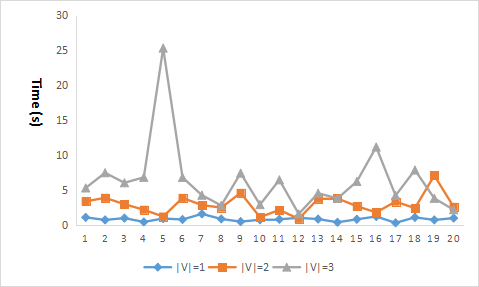
\includegraphics[width=7cm]{chapter04/time_4_12.png}
%	}
%	\subfigure[$\CTLsnf$子句的个数]{
%		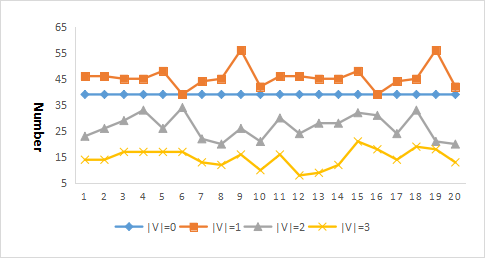
\includegraphics[width=7cm]{chapter04/number-4-12.png}
%	}
%	\caption{$\varphi_i=12$时的计算结果}
%	\label{chapter04:fig:for12}
%\end{figure*}
%
%\begin{figure*}[!htb]
%	\centering
%	\subfigure[计算遗忘需要的CUP时间]{
%		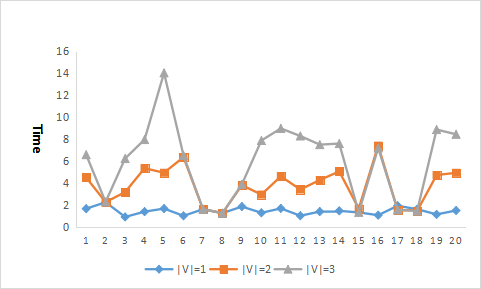
\includegraphics[width=7cm]{chapter04/time_4_16.png}
%	}
%	\subfigure[$\CTLsnf$子句的个数]{
%		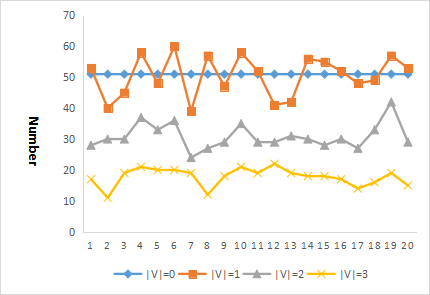
\includegraphics[width=7cm]{chapter04/number-4-16.png}
%	}
%	\caption{$\varphi_i=16$时的计算结果}
%	\label{chapter04:fig:for16}
%\end{figure*}
%
%\subsection{SNC计算结果分析}
%这部分实验分析使用基于遗忘的方法计算$\CTL$公式的SNC,分为两组实验:分别计算经典命题公式和$\CTL$公式的SNC,即:计算$q$在$V$和$\varphi \wedge q$上的SNC($\CTLforget(\varphi\wedge q, \Var(\varphi)-V \cup \{q\})$),其中$V\subseteq \Var(\varphi)$、$q\in \Var(\varphi\wedge q)-V$。
%这些公式$\varphi$都是随机生成的定义在原子命题集合$\Ha$上的公式、$V$也是在计算过程中随机生成的、$q\not \in \Var(\varphi)$是一个固定的原子命题且$|\Ha|=50$。
%
%首先测试随机3-CNF命题公式。令$|V|$的取值范围为$\{5,10,\dots, 40,45\}$,3-CNF公式的子句个数$nc$范围为$\{10,15,\dots, 45,50\}$。
%在每种情形当中,计算20个随机实例$(\varphi,q,V)$:$\varphi$为$\Ha$上的公式,且$V\subseteq \Var(\varphi)$。
%计算SNC的平均CPU时间如图\ref{chapter04:fig:ProTime}所示。
%
%\begin{figure*}[!htb]
%	\centering
%	\subfigure[平均CPU时间(s)]{
%		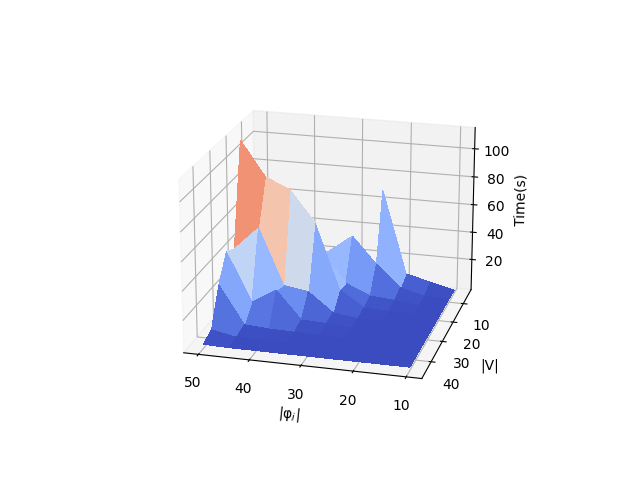
\includegraphics[width=7.5cm]{chapter04/PRototalAveTime.png}
%	}
%	\subfigure[$|V|=25$时所使用CPU时间箱线图 % and $|\varphi|~\in~ \{10, 15,\dots, 50\}$
%	]{
%		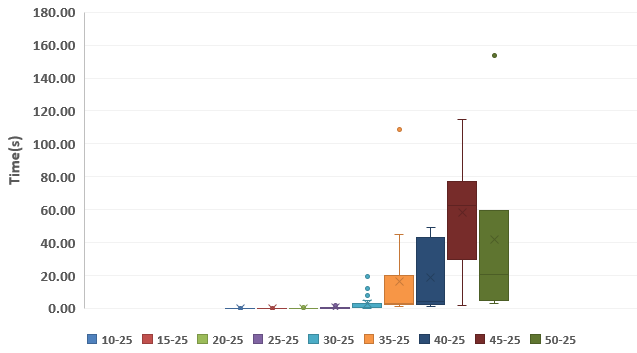
\includegraphics[width=7cm]{chapter04/ProBox(10-50)_25.png}
%	}
%	\caption{%The performances of computing SNC in PL.
%		计算3-CNF公式的SNC所需的CPU时间情况}
%	\label{chapter04:fig:ProTime}
%\end{figure*}
%
%
%从图\ref{chapter04:fig:ProTime}(a)可看出,随着$|\varphi|$增大或$|V|$的减小时间消耗越大。
%直观地说,越大的$|\varphi|$或者越小的$|V|$意味着$\CTLforget(\varphi, \overline{V})$更难计算。
%这与上一小节中的结论相符合。
%图\ref{chapter04:fig:ProTime}(b)展示了当$|V|= 25$、$nc\in \{10,15,\dots, 45, 50\}$时20个随机实例的箱线图。
%这同样证明了$nc$越大SNC越难计算。
%
%
%其次,测试具有如下形式的$\CTL$公式的SNC的计算:
%$$\varphi_1 \wedge \ALL \NEXT \varphi_2 \wedge \EXIST\NEXT \varphi_3$$
%其中$\varphi_i$($i=1,2,3$)为随机产生的定义在$\Ha$上的3-CNF公式,且满足$|\varphi_1|=|\varphi_2|=|\varphi_3|$。
%在这种情形下,每个实例$(\varphi, q, V)$是随机产生的,其中$\varphi=\varphi_1 \wedge \ALL \NEXT \varphi_2 \wedge \EXIST\NEXT \varphi_3$、$V\subseteq \Var(\varphi)$、$|\varphi|\in \{5,6,\dots, 13,14\}$、且$|V|\in \{15,16,\dots, 23,24\}$。
%值得注意的是在实例$(\varphi, q, V)$中,$q$可能没有在$V$和$\varphi\wedge q$上的SNC。
%
%图\ref{chapter04:fig:CtlTime}(a)展示了每种情形计算40个实例的SNC的平均CPU时间。与命题公式的情形相似,越大的$|\varphi|$或者越小的$|V|$意味着$\CTLforget(\varphi, \overline{V})$更难计算。
%此外,图\ref{chapter04:fig:CtlTime}(b)展示了每种情形下40个实例中SNC存在的占比,即:$|\varphi|$越小或者$|V|$越小则SNC存在的占比越大。特别地,当$|\varphi_i|=5$且$|V|=16$时,SNC存在的占比为80\%。
%
%
%
%\begin{figure*}[!htb]
%	\centering
%	\subfigure[平均CPU时间(s)]{
%		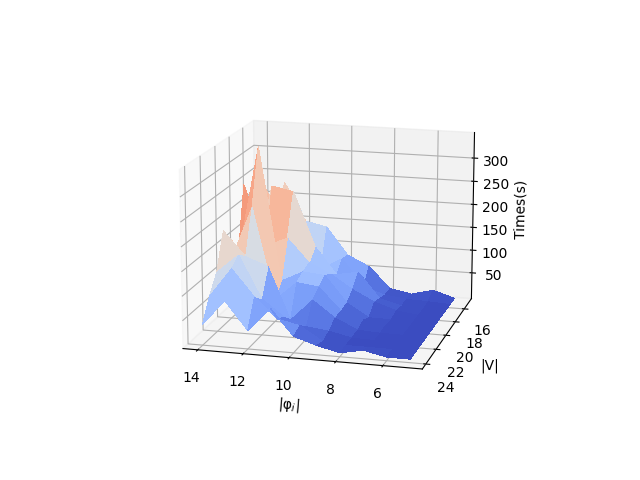
\includegraphics[width=7cm]{chapter04/totalAveTime.png}
%	}
%	\subfigure[SNC存在的占比(\%)]{
%		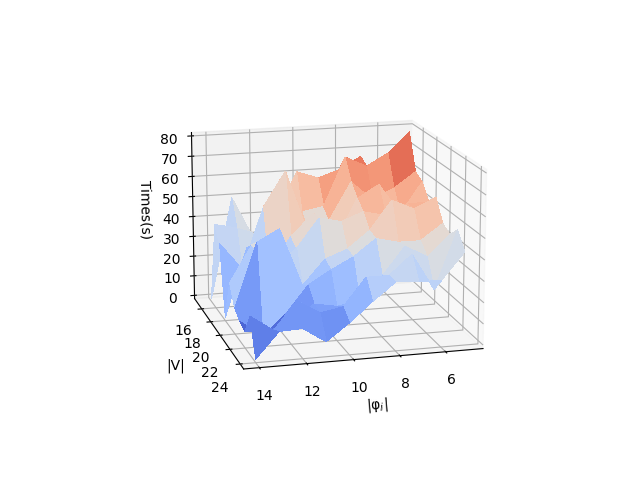
\includegraphics[width=7cm]{chapter04/numPercent.png}
%	}
%	\caption{$\CTL$下计算SNC的性能情况.}
%	\label{chapter04:fig:CtlTime}
%\end{figure*}
%
%综上所述,算法\ref{alg:compute:forgetting:by:Resolution}大多数情况下能计算出SNC(WSC),且当需要遗忘的原子个数很少或公式长度较小的时候计算效率很高。

\section{本章小结}\label{chapter04-conclusion}

本章探索了如何使用Zhang等人提出的归结系统计算$\CTL$下的遗忘。为此,首先使用Zhang提出的转换规则将$\CTL$公式转换成$\CTLsnf$子句的集合,这一步骤在第\ref{chapter02}章讲述$\CTL$的标准形式时已经给出。基于此,使用归结规则在要遗忘的原子命题集合上做穷尽的归结。然后提出几个互模拟等价的消除索引的等式消除索引,并提出一般化的Ackermann引理用于移除一些新引入的原子命题。最后,给出了计算遗忘的算法,并分析了算法的复杂性,表明了使用该算法计算遗忘的时间和空间复杂性关于公式和要遗忘的原子命题的个数是指数时间的。

